\section{Segmentation of the MILP problem}
\label{section:segment}


\subsection{Introduction}
The MILP model described in section \ref{section:modelingbasic} is sufficient to solve the trajectory planning problem for short flights with few obstacles. However, it scales poorly when the duration of the flight or the amount of obstacles is increased. Mixed-Integer programming belongs to the ``NP-Complete'' class of problems \cite{DBLP:conf/coco/Karp72}. This is a class of problems which is considered very hard to solve. As the amount of integer variables grows, the time needed to solve the problem increases exponentially. An integer variable is needed for every edge of every polygon, for every time step. By reducing both the amount of time steps needed and obstacles that need to be modeled, the execution time can be reduced dramatically. \\
The key insight that allows my algorithm to scale well beyond what's usually possible is that the path trajectory not need to be solved all at once. If the trajectory planning problem can be split into many different subproblems, each subproblem becomes easier to solve. The solution for each subproblem is a small part of the final trajectory. By solving theses subproblems sequentially, the final trajectory can gradually be constructed. \\
While diving the problem into subproblems does make things much easier to solve, it also has an important down side: Finding the fastest trajectory can no longer be guaranteed. Smaller subproblems make it easier to find a solution, but fundamentally the problem of finding the optimal trajectory is still just as hard. The necessary trade-off for better performance is that the optimal trajectory will likely not be found. Luckily, the optimal trajectory is often not required in navigation. A reasonably good trajectory will do.

\subsubsection{The importance of convexity}
While the worst case time needed to solve a MILP problem increases exponentially with the amount of integer variables, this is not the most useful way to measure the difficulty of a problem. Modern solvers are heavily optimized and are able to solve certain problems with many integer variables much faster than others. The key difference is the convexity of the solution space. Just like a circle is the solution space for ``all points a certain distance away from the center point'', the constraints used to model the trajectory planning problem form some geometric shape with a dimension for every variable. \\
When only linear constraints with real values are used, the solution space will always be convex. It is this convexity that makes a standard linear program easy to solve. When integer variables are introduced, it is possible to construct solution spaces which are not convex. As the solution space becomes less and less convex, the problem becomes harder to solve. Integer variables can be seen as a tool which allows non-convex solution spaces to be modeled. When trying to improve the difficulty of a problem, the actual goal is making the problem more convex (or smaller, which always helps). Reducing the amount of integer variables is only a side effect. \\
This insight is critical when determining how to divide the trajectory problem into smaller subproblems, and which obstacles are important for each subproblem.
\subsubsection{General Algorithm Outline}
\begin{algorithm}
\caption{General outline}
\label{alg:outline}
\begin{algorithmic}[1]
\State $T \leftarrow \{\}$ \Comment{The list of trajectories solved so far}
\State $path \leftarrow$ \Call{Theta*}{$scenario$}
\State $events \leftarrow$ \Call{FindCornerEvents}{$path$}
\State $segments \leftarrow$ \Call{GenSegments}{$path$, $events$}
\ForEach {$segment \in segments$}
\State \Call{UpdateStartState}{$segment$}
\State \Call{GenActiveRegion}{$scenario$, $segment$}
\State $T \leftarrow T \cup \{$ \Call{SolveTrajectory}{$segment$} $\}$
\EndFor
\State $result \leftarrow $\Call{MergeTrajectories}{$T$}
\end{algorithmic}
\end{algorithm}
The algorithm I developed consists of two phases.\\
In the first phase, information is gathered about the trajectory planning problem. The Theta* algorithm is used to construct an initial path from the start to the goal position. Unlike a trajectory, a path is not time-dependent and does not take dynamic properties into account. This makes a path much easier to calculate than a trajectory. While the Theta* path is not suitable to describe the movements of a UAV, it contains useful information about the trajectory we want to calculate. More specifically, the turns in the Theta* path are used to generate path segments. Each path segment contains the information needed to construct a MILP subproblem. \\
In the second phase, each path segment considered sequentially. First, for all but the first segment,


\subsection{Finding the initial path}

The first issue is that because the goal cannot be reached immediately, the goal function for the MILP problem needs to change.  \\
One option is to simply get as close as possible to the goal during each segment. Because the distance that can be traveled during a segment is limited, the amount of obstacles that need to be modeled is also limited. This works well when the world is very open with little obstacles. However, this greedy approach is prone to getting stuck in dead ends in more dense worlds like cities.
\\
The second option is finding a complete path using a method that's easier to compute. An algorithm like A* can be used to find a rough estimation for the path. This A* path is the shortest path, but does not take constraints or the characteristics of the vehicle into account. A very curvy direct path may be the shortest, but a detour which is mostly straight and allows for higher speeds may actually be faster. 
\\
It is possible to use more advanced algorithms that model more of the constraints. This will significantly improve the execution time of the MILP solver and quality of the solution, but it will also come at a performance cost. A balance needs to be found between the execution time of the preprocessing step and that of the MILP solver. The preprocessing step needs to do just enough so the solver can find a good solution in an acceptable amount of time. 
\\
I have decided to use Theta*. This is a variant  of A* that allows for paths at arbitrary angles instead of multiples of 45 degrees. The main reason for this is that it eliminates the ``zig zags'' that A* produces. This makes the next step of the preprocessing much easier. The left image in figure \ref{fig:pre-1-2} shows the result of the Theta* algorithm.\\



%\subsection{Introduction}
%TODO:REWRITE
%Key to making MILP scale is dividing the problem into smaller pieces. Goal cannot be reached in a single segment, so needs to be guided some other way. Need to consider that multiple corners in single segment is problematic, so segments should minimize the amount of corners. Will use theta* and detect corners, use corners to construct segments.\\
%Smaller segments allow lower upper bound on time needed, obstacles still an issue. Maximum possible distance vehicle can travel is first approximation, but still not enough in dense cities. Need to significantly cut down on amount of obstacles safely. Will demonstrate that not every obstacle is equally important, how to find the important obstacles and safely compress other obstacles using genetic algorithm.\\
%Stress that the solution chosen can be swapped out. What's written here is one option.
%
%
%
%
%%Short paths can be solved directly, but longer paths with a large amount of obstacles nearby take an extremely long time to solve. A solution to this problem is to divide the path into smaller segments. Solving the smaller segments is proportionally disproportionately easier than solving the full path, but at the cost of optimality and stability.\\
%\subsection{Guiding the segmented path}
%The first issue is that because the goal cannot be reached immediately, the goal function needs to change.  \\
%One option is to simply get as close as possible to the goal during each segment. Because the distance that can be traveled during a segment is limited, the amount of obstacles that need to be modeled is also limited. This works well when the world is very open with little obstacles. However, this greedy approach is prone to getting stuck in dead ends in more dense worlds like cities.
%\\
%The second option is finding a complete path using a method that's easier to compute. An algorithm like A* can be used to find a rough estimation for the path. This A* path is the shortest path, but does not take constraints or the characteristics of the vehicle into account. A very curvy direct path may be the shortest, but a detour which is mostly straight and allows for higher speeds may actually be faster. 
%\\
%It is possible to use more advanced algorithms that model more of the constraints. This will significantly improve the speed and quality of the constraint optimization step, but it will also come at a performance cost. A balance needs to be found between the preprocessing step and the constraint optimization step. The preprocessing step needs to do just enough so the optimization step can be solved in an acceptable amount of time. 
%\\
%
%
%heuristic
%indexed obstacles
%possible position: first fuzzy collision, after: LOS check with last point
%line of sight: first bounding box overlap, only after LOS
%
%
%I have decided to use Theta*. This is a variant  of A* that allows for paths at arbitrary angles instead of multiples of 45 degrees. The main reason for this is that it eliminates the ``zig zags'' that A* produces. This makes the next step of the preprocessing much easier.\\
\subsubsection{Theta* implementation}
\begin{figure}
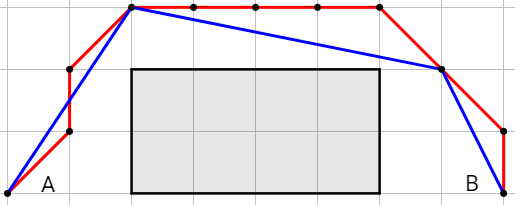
\includegraphics[width=\textwidth]{a_theta_star_comp3}
\label{figure:thetastarcompare}
\end{figure}

\subsubsection{Theta* optimizations}
heuristic \\
indexed obstacles \\
possible position: first fuzzy collision, after: LOS check with last point \\
line of sight: first bounding box overlap, only after LOS \\

\subsubsection{Scalability of Theta*}
TODO: REWRITE... KEEP?
Theta* provides the information that makes it possible to make MILP fast, but Theta* in itself is intractable. Why is this not simply moving the issue?\\
Theta* is indeed intractable, but still much better than MILP. Holomomic vs non-holonomic. Concept of navigation mesh as part of map, often used in video games to allow AI to navigate large worlds. Also same concept behind PRM. Only needs to pre precomputed once per map. Can serve as heuristic for Theta*, or completely replace it.


\subsection{Detecting corner events}
With an initial path generated, the next problem is dividing it into segments. Dividing the path into equal parts presents problems, because when solving each segment, the solver has no knowledge of what will happen in the next segment. This is especially problematic when the vehicle needs to make a tight corner. If the last segment ends right before the corner, it may not be possible to avoid a collision. Because of this, corners need to be taken into account when generating the segments. The right image in figure \ref{fig:pre-1-2} shows the transitions between segments as green circles.\\
In Euclidian geometry, the shortest path between two points is always a straight line. When polygonal obstacles are introduced between those points, the shortest path will be composed of straight lines with turns at one or more vertices of the obstacles. The obstacle that causes the turn will always be on the inside of the corner. This shows why corners are important for another reason: They make the search space non-convex. For obstacles on the outside of the corner it is possible to constrain the search space so it is still convex, but this is not possible for obstacles on the inside of a corner.\\
Because of these reasons, isolating the corners from the rest of the path is advantageous. With enough buffer before the corner, the vehicle is much more likely to be able to navigate the corner successfully. It also means that the computationally expensive parts of the path are as small as possible while still containing enough information for fast navigation through the corners.
\\
The reason for using Theta* becomes clear now. Every single node in the path generated by the algorithm is guaranteed to be either the start, goal or near a corner. A corner can have more than one node, so nodes which turn in the same direction and are close to each other are grouped together and considered part of the same corner. For each corner, a corner event is generated.

\subsubsection{Algorithm Implementation}
code \\
parameter tolerance, link to acc distance\\
\subsubsection{Tight Coupling with Theta*}
This algorithm relies on assumptions from Theta*, so if algorithm changes, this will need to be updated.


\begin{figure}[!t]
    \centering
    \begin{subfigure}[t]{0.47\textwidth}
        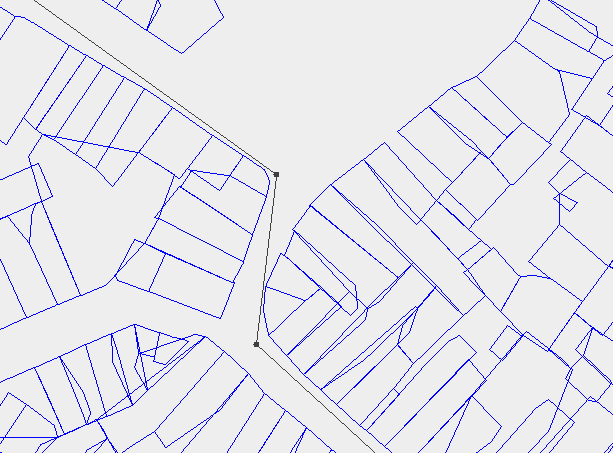
\includegraphics[width=\textwidth]{img/pre1}
    \end{subfigure}
    \hfil
    \begin{subfigure}[t]{0.47\textwidth}
        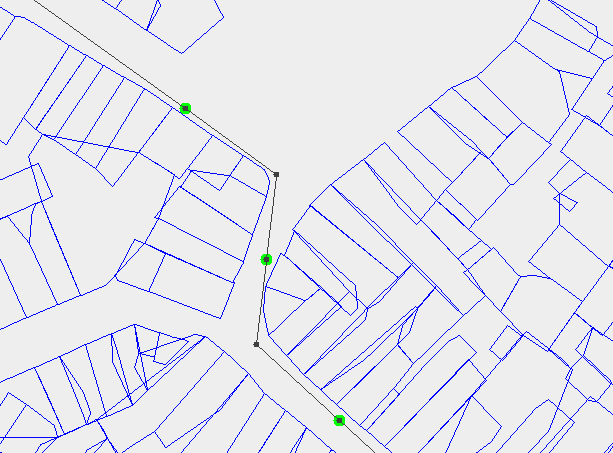
\includegraphics[width=\textwidth]{img/pre2}
    \end{subfigure}
    \caption{The left image shows the results after the Theta* algorithm has executed. The blue shapes are obstacles, while the gray line is the Theta* path. The right image shows the results after the path is segmented. Extra nodes have been added to the Theta* path, as marked by the green circles. These circles depict the transitions between segments.}\label{fig:pre-1-2}
\end{figure}

\begin{figure}[!t]
    \centering
    \begin{subfigure}[t]{0.47\textwidth}
        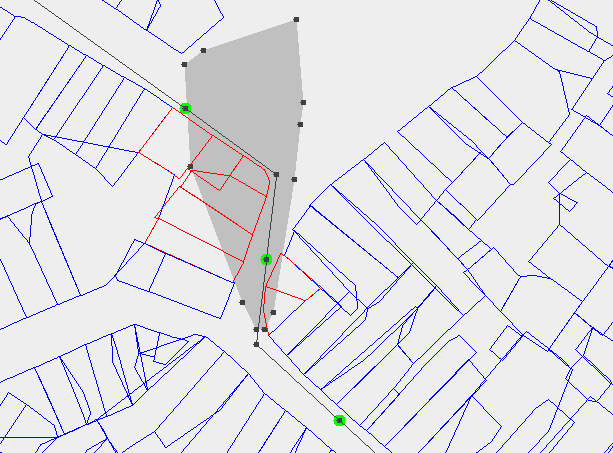
\includegraphics[width=\textwidth]{img/pre3}
    \end{subfigure}
    \hfil
    \begin{subfigure}[t]{0.47\textwidth}
        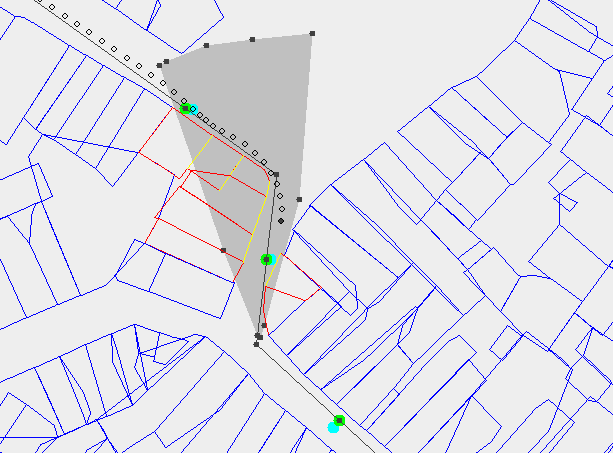
\includegraphics[width=\textwidth]{img/pre4}
    \end{subfigure}
    \caption{The left image shows the result after the genetic algorithm has executed. The obstacles in red have been selected to be modeled in the MILP problem. The dark grey shape is the convex allowed region generated by the genetic algortihm. Note how it does not overlap with any of the blue obstacles. The right image shows the final result. The trail of circles show the path of the vehicle up to the current time step, which is represented by the filled circles. The red and yellow colors depict the same information as in figure \ref{fig:obs}}\label{fig:pre-3-4}
\end{figure}

\subsection{Generating path segments}
\begin{algorithm}
\caption{Generating the segments}
\label{alg:segments}
\begin{algorithmic}[1]
\Function{GenSegments}{$path$, $events$}
\State $segments \leftarrow \{\}$
\State $catchUp \leftarrow true$
\State $lastEnd \leftarrow path(0)$
\For {$i \gets 0, |events| - 1 $}
\State $event \leftarrow events(i)$
\If{$catchUp$}
	%\State $segStart \leftarrow $ \Call{ExpandBackw}{$event.start$}
	%\State \Call{AddSegments}{$lastSegEnd$, $segStart$}
	%\State $lastSegEnd \leftarrow segStart$ 
	\State expand $event.start$ backwards
	\State add segments from $lastEnd$ to $event.start$
	\State $lastEnd \leftarrow event.start$
\EndIf
\State $nextEvent \leftarrow events(i+1)$
\If{$nextEvent.start$ is close to $event.end$}
	\State $mid \leftarrow$ middle between $event$ \& $nextEvent$
	\State add segment from $lastEnd$ to $mid$
	\State $lastEnd \leftarrow mid$
	\State $catchUp \leftarrow false$
\Else
	\State expand $event.end$ forwards
	\State add segment from $lastEnd$ to $event.end$
	\State $lastEnd \leftarrow event.end$
	\State $catchUp \leftarrow true$
\EndIf
\EndFor
\State add segments from $lastEnd$ to $path(|path|-1)$
\Return $segments$
\EndFunction
\end{algorithmic}
\end{algorithm}



%These corner events are in turn grown outwards to cover the approach and departure from the corner. How much depends on the maximum acceleration of the vehicle. As a rule of thumb: If the vehicle can come to a complete stop from its maximum speed before the corner, it can also successfully navigate that corner. When corners appear in quick succession, their expanded regions may overlap. In that case, the middle between those corners is chosen. Long, straight sections are also divided into smaller path segments.\\
%One of the main goals of segmenting the path is to reduce the amount of obstacles. This means that every segment has a set of obstacles associated with it, being the obstacles that need to be modeled in the optimization step. Not only the obstacle that ``causes'' the corner is important, but obstacles which are nearby are important as well. Obstacles on the outside of the corner also may play a role in how the vehicle approaches the corner. To find all potentially relevant obstacles, the convex hull of the (Theta*) path segment is calculated and scaled up slightly. Every obstacle which overlaps with this shape is considered an active obstacle for that path segment. The convex hull step ensures that all obstacles on the inside of the corner are included, while scaling it up will cover any restricting obstacle on the outside of the corner.

\subsubsection{Segment Generation Algorithm}
code \\
approachmargin \\
maxtime \\
step by step figures with explanation? 
\subsubsection{Segment data}
relevant points: pre path + stop point going in + stop point at finish. image with points clearly labeled \\
convex hull: quickhull. source + image for demo \\
note: only when about to be solved!
\subsection{Generating the active region for each segment}
One of the main goals of segmenting the path is to reduce the amount of obstacles. Every segment has a set of active obstacles associated with it, being the obstacles that need to be modeled for the solver. Not only the obstacle that ``causes'' the corner is important, but obstacles which are nearby are important as well. Obstacles on the outside of the corner also may play a role in how the vehicle approaches the corner. To find all potentially relevant obstacles, the convex hull of the (Theta*) path segment is calculated and scaled up slightly. Every obstacle which overlaps with this shape is considered an active obstacle for that path segment. The convex hull step ensures that all obstacles on the inside of the corner are included, while scaling it up will cover any restricting obstacle on the outside of the corner.\\
The inactive obstacles also need to be represented. To do this, a convex polygon is constructed around the path. This polygon may intersect with the active obstacles (since they will be represented separately), but may not intersect any other obstacle. The polygon is grown using a genetic algorithm. Genetic algorithms are inspired by natural selection in biology. A typical genetic algorithm consists of a population of individuals, a selection strategy and one or more operators to generate offspring. In each generation, the operators are applied on the population to produce offspring. These operators usually have a random element and are responsible for exploration of the search space. The selection strategy determines, often based on a fitness function, which individuals survive and form the population for the next generation. Selection is responsible for convergence towards fitter individuals, limiting how much of the search space is evaluated. \\

\subsubsection{Implementation of the genetic algorithm}
\begin{algorithm}
\caption{Genetic Algorithm}
\label{alg:ga}
\begin{algorithmic}[1]
\Function{GenActiveRegion}{$scenario$, $segment$}
\State $pop \leftarrow $ \Call{SeedPopulation}{}
\For {$i \gets 0, N_{gens} $}
\State $pop \leftarrow pop \cup $ \Call{Mutate}{$pop$}
\State \Call{Evaluate}{$pop$}
\State $pop \leftarrow $ \Call{Select}{$pop$}
\EndFor
\Return \Call{BestIndividual}{$pop$}
\EndFunction
\Function{Mutate}{$pop$}
\ForEach {$individual \in pop$}
\State add vertex with probability $p_{add}$
\State OR remove vertex with probability $p_{remove}$
\ForEach {$gene \in individual.chromosome$}
\State randomly move vertex by at most $\Delta_{nudge}$
\If{new polygon is legal}
\State update polygon
\Else
\State try again at most $N_{attempts}$ times
\EndIf
\EndFor
\EndFor
\Return \Call{BestIndividual}{$pop$}
\EndFunction
\end{algorithmic}
\end{algorithm}

Alg. \ref{alg:ga} shows our implementation. In our implementation, each individual in the population represents a single legal polygon. A legal polygon is convex, does not self-intersect, does not overlap with inactive obstacles and contains every node in the Theta* path for that specific segment. The latter requirement prevents the polygon from drifting off. Each individual has a single chromosome, and each chromosome has a varying number of genes. Each gene represents a vertex of the polygon.\\
The only operator is a mutator (line 4). Contrary to how mutators usually work, the mutation does not change the original individual. This means that the every individual can be mutated in every generation, since there is no risk of losing information. This mutator can add or remove vertices of the polygon by adding or removing genes (lines 12-13), but only if the amount of genes stays between $N_{genes,min}$ and $N_{genes,max}$. The mutator attempts to nudge every vertex/gene to a random position at most $\Delta_{nudge}$ away (line 15). If the resulting polygon is not legal, it retries at most $N_{attempts}$ times (line 16-19). \\
Tournament selection is used as the selector, with the fitness function being the surface area of the polygon (line 5-6). Fig. \ref{fig:pre-comp} Shows the active obstacles in yellow and red, as well as the polygon generated by the genetic algorithm in dark gray.\\


library \\
tournament selection \\
offspring generation: mutate only \\
initial population \\
chromosome/gene description \\
fitness function \\
validation \\
parameters \\
obstacle selection based on path length? \\


